\documentclass{beamer}
\usepackage{graphicx}
\usepackage[utf8]{inputenc}
\usepackage[T1]{fontenc} 

\usetheme[hideallsubsections]{PaloAlto}

\usepackage{tikz}
\usepackage{verbatim}
\usepackage{tabularx}
\usepackage{array}

% vertically centering in tables when X
\renewcommand{\tabularxcolumn}[1]{>{\small}m{#1}}
\usepackage{makecell}
\usepackage{color}
\usepackage{diagbox}

\usepackage[french,english]{babel}
\usepackage{lmodern} 


% \setbeamertemplate{sections in toc}[sections numbered]
% \usetikzlibrary{arrows,shadows,shapes,backgrounds,positioning}
% \beamertemplatetransparentcovered

% insert page number in Beamer Navigation Bars
\addtobeamertemplate{navigation symbols}{}{%
    \usebeamerfont{footline}%
    \usebeamercolor[fg]{footline}%
    \hspace{1em}%
    \insertframenumber/\inserttotalframenumber
}

% set head height
\makeatletter
\setlength{\beamer@headheight}{0.7cm}
\makeatother


\title[]{Licensing in a software project} 
\author{Rémi Boulle  \href{mailto:mail@remiboulle.fr}{mail@remiboulle.fr}}
\date{}       
\institute{}        

\begin{document}

% section titles in a special slide
\AtBeginSection[]{
  \begin{frame}
  \vfill
  \centering
  \begin{beamercolorbox}[sep=8pt,center,shadow=true,rounded=true]{title}
    \usebeamerfont{title}\insertsectionhead\par%
  \end{beamercolorbox}
  \vfill
  \end{frame}
}

%%%%%%%%%%%%%%%%
% Title
%%%%%%%%%%%%%%%%

\begin{frame}
  \titlepage
\end{frame}


%\section{Objectifs}

\begin{frame}
\frametitle{Your goal}
\begin{alertblock}{Main goal}
  Acquire and strengthen your expertise on free software licenses
\end{alertblock}


  \begin{itemize}
  \item History and context
  \item Different categories of licenses
  \item Diffusivity and compliance rules
  \item Auditing your project
  \item Free software economics
  \end{itemize}
\end{frame}

%%%%%%%%%%%%%%%%%%%%%%%%%%%%%%%%%%%%%%%%%%%%%%%%%%%%%%%%
% Context, vocabulary
%%%%%%%%%%%%%%%%%%%%%%%%%%%%%%%%%%%%%%%%%%%%%%%%%%%%%%%%

\section{Context}

\begin{frame}{History}
  \begin{itemize}
  \item GNU project in 1984 by Richard Stallman (RMS)
  \item GPLv1 : 25th of february 1989
  \item la technique est un moyen pour atteindre un but social
  \item 1991 : Minix kernel (\textit{just a hobby, won't be big and professional like gnu} by Linus Torvalds (LT)
  \item 1995 : Red Hat (Nasdaq in 1999), Apache license
  \item 1998 : release of Netscape source-code (fight back IE. Free the lizard, mozilla)
  \item 1998 : "Free software" versus "Open Source Software" (OSI). Rebranding the free software movement to emphasize the business potential ? 
  \end{itemize}
\end{frame}


\setbeamertemplate{background canvas}{\centering\includegraphics
   [width=\paperwidth]{images/rms.jpg}}
\begin{frame}[plain]%{RMS}
%  
\note{RMS}
\end{frame}
\setbeamertemplate{background canvas}{}


\setbeamertemplate{background canvas}{\centering\includegraphics
   [height=\paperheight]{images/LinusTorvalds.jpg}}
\begin{frame}[plain]%{LT}
%  
\note{Linus Torvalds}
\end{frame}
\setbeamertemplate{background canvas}{}

\setbeamertemplate{background canvas}{\centering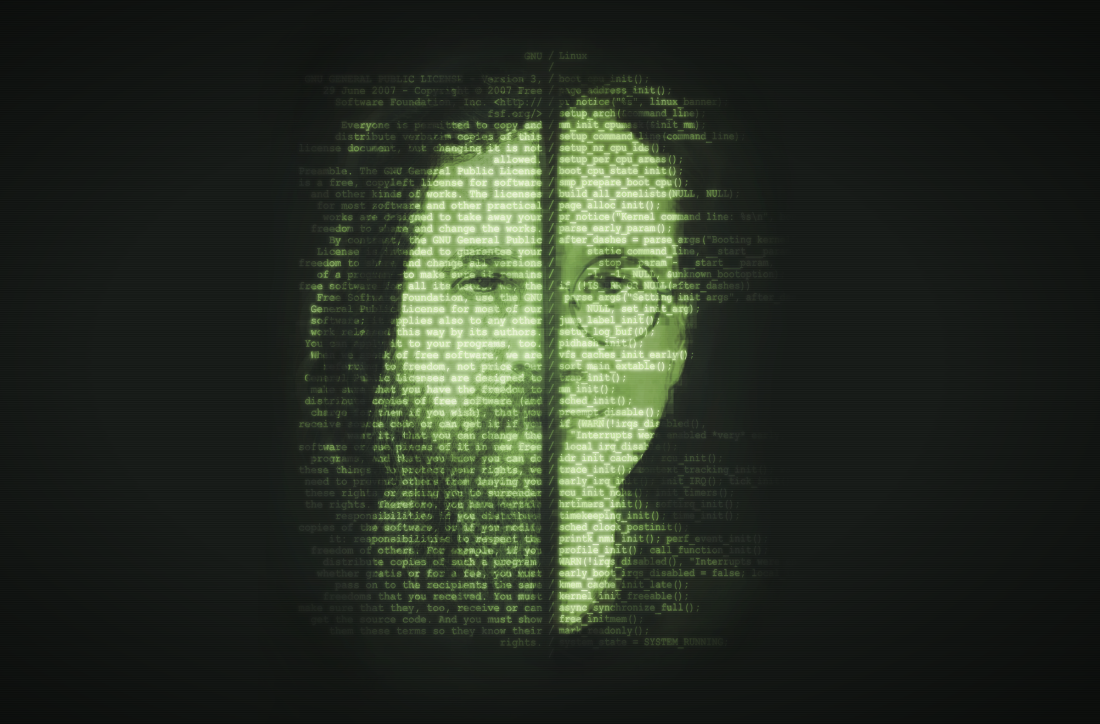
\includegraphics
   [height=\paperheight]{images/gnu-linux_wallpaper_tb_david_revoy.png}}
\begin{frame}[plain]%{LT}
%  
\note{GNU/Linux}
\end{frame}
\setbeamertemplate{background canvas}{}

\begin{frame}{Communities and organizations}

  \begin{block}{International}
    Free Software Fondation : \url{https://www.fsf.org/}

    Open Source Initiative : \url{https://opensource.org/}

    Linux Fondation : \url{https://www.linuxfoundation.org/}

    Debian, python, Ubuntu, KDE... communities
  \end{block}

\pause

  \begin{block}{Europe}
    France : CNLL : \url{http://cnll.fr/}, April : \url{https://april.org/}, Framasoft : \url{https://framasoft.org/}

    
  \end{block}
\end{frame}


\begin{frame}{Free and/or Open Source}

  \begin{block}{Free Software}
    Social movement, user's essential freedom, free as in freedom. \textit{"political and ethical choice asserting the right to learn, and share what we learn with others"}
  \end{block}

\textit{"All freedoms depend on freedom of information and are not more important than other fundamental freedoms, but as life's practices change over to the computer, it will be needed to maintain other freedoms". (RMS)}

  \begin{block}{Open Source}
    Concerned solely with licensing of source code (not tivoization) :  \textit{"I think ideology sucks"} (Linus Torvalds), pragmatism.
  \end{block}

We are always the ideologue of someone... Outdated debate ?
\end{frame}

\section{Vocabulary}


\begin{frame}{Vocabulary}

  \begin{itemize}
  \item \textbf{proprietary software} but all software have authors.
  \item \textbf{Copyleft} : \textit{we give rights}, all modified and extended versions of the program must be free as well, under the same terms. You cannot add restrictions to deny other people freedoms.
  \item \textbf{Copyright} :  legal term describing rights given to creators for their works. Under the Berne Convention, everything written is automatically copyrighted from whenever it is put in fixed form
  \item Copyleft is not opposed to Copyright but a clever hack
  \end{itemize}
\end{frame}

\section{Copyright}

\begin{frame}{Copyright}

With the creation authors obtain intellectual property rights.

  \begin{itemize}
  \item Economic right : right to exploit the work
    \begin{itemize}
    \item permit or prohibit the fixation and reproduction of his or her work
    \item translation, arrangement, adaptation and alteration of the work
    \item distribution of the original or copies
    \item Related rights
    \end{itemize}
  \item Moral right
    \begin{itemize}
    \item right to protect their personal connection with the work
    
    \end{itemize}
  \end{itemize}

 \begin{alertblock}{Copyleft is not opposed to copyright}
    Free and proprietary software \textit{copyright}.
  \end{alertblock}

  \begin{alertblock}{EU directive}
    Only the expression of a computer program is protected and that ideas and principles which underlie any element of a program, including those which underlie its interfaces, are not protected by copyright.
  \end{alertblock}

\end{frame}

%%%%%%%%%%%%%%%%%%%%%%%%%%%%%%%%%%%%%%%%%%%%%%%%%%%%%%%%
% Proprietary software
%%%%%%%%%%%%%%%%%%%%%%%%%%%%%%%%%%%%%%%%%%%%%%%%%%%%%%%%

\section{Proprietary}

\begin{frame}{Proprietary software}
  General principle : limitations against use, distribution and modification. Used by end-users under predefined conditions.

  \begin{alertblock}{Definition : proprietary software}
    Software who limits one or more of the 4 freedoms of free software.    
  \end{alertblock}

\pause

  \begin{block}{Michel Rocard, 2002, patent battle : 648 no, 14 yes, 18 abs}
   \textit{Creation, freedom, innovation were on the side of free software. The pursuit of profit, and above all the rent, the desire to restrict competition, and to restrain the external innovations, were on the side of big industry.}
  \end{block}
\end{frame}

\begin{frame}{Governance ?}
  
\textit{If you can not enter through the door, go in through the window !}

Who is in charge of governing which free software project ? Just asking...

\end{frame}

%%%%%%%%%%%%%%%%%%%%%%%%%%%%%%%%%%%%%%%%%%%%%%%%%%%%%%%%
% Free software
%%%%%%%%%%%%%%%%%%%%%%%%%%%%%%%%%%%%%%%%%%%%%%%%%%%%%%%%

\section{Free Software}


\begin{frame}{Free Software}

  \begin{alertblock}{General principle}
    \textit{Free as in free speech, not as in free beer}. Source code is free.
  \end{alertblock}
  Their main difference : modalities of redistribution
  \begin{enumerate}
  \item redistribution but code must stay free : user's should receive a copy of the code under the same terms
  \item redistribution but code must stay free : user's are not guaranteed to receive a copy
  \end{enumerate}

  \begin{alertblock}{Definition : free software}
   A program is free software if the \textbf{program's users} have the four essential freedoms.
  \end{alertblock}
  
\end{frame}


\begin{frame}{freedom 0 : freedom to run the program}
  \begin{itemize}
  \item Absolute freedom to run by anyone without \textbf{any} restriction
  \item A work produced with a free software doesn't have to be free
  \item Some production made by a free software could been seen as a derivative work (compiler mostly).
  \item What about SaaS ?
  \end{itemize}

  \begin{alertblock}{Principe}
     it is the user's purpose that matters, not the developer's one.
  \end{alertblock}
  
  Quick question : Is JSON license free ? \url{http://www.json.org/license.html}

\end{frame}


\begin{frame}{freedom 1 : freedom to study}
  \begin{itemize}
  \item study without any obstacles (technicals, rights...)
  \item includes the freedom to use your changed version in place of the originalfreedom d'étude
  \item Not obliged to give source code with binaries (by pragmatsim)
  \item Source code should be made available for free or at a low cost
  \item Source code available for at leats 3 years (GPLv3)
  \end{itemize}
  \begin{alertblock}{Principe}
    Again, it is the user's purpose that matters, not the developer's one
  \end{alertblock}
\end{frame}


\begin{frame}{freedom 2 : freedom to modify}
  \begin{itemize}
  \item absolute freedom. Only restrictions when distribution.
  \item Preserve copyritht ownership (Berne convention)
  \item Identify  contributions
  \end{itemize}
\begin{alertblock}{Principe}
    Always, it is the user's purpose that matters
  \end{alertblock}
\end{frame}

\begin{frame}{freedom 3 : freedom to redistribute}

Anyone, anywhere (export control, trade sanctions...)

  \begin{itemize}
  \item Conditions of redistribution : main difference between all free software licenses :
    \begin{itemize}
    \item \textbf{Strong Copyleft}
    \item \textbf{Weak Copyleft}
    \item \textbf{Copyfree}
    \end{itemize}
  \item Always identify contributors (Berne convention)
  \item Preserve original authors' reputation
  \end{itemize}
\begin{alertblock}{Principle}
    User's purpose again and mostly necessary condition for the three others freedoms.
  \end{alertblock}

\begin{alertblock}{When does license apply ?}
\textbf{Redistribution triggers !}
 \end{alertblock}
 
 Exception : APGL where it is 
\end{frame}

\section{TP1}

\begin{frame}{Study the four "freedoms" of proprietary softwares}
  By groups of 3, in 45 minutes :
  \begin{itemize}
  \item open a framapad
  \item analyse for each of the 4 freedoms their transposition with proprietary software.
  \item the sharing of works will be made on a common pad
  \end{itemize}

  \begin{alertblock}{General guideline}
	Always give relevant references 
  \end{alertblock}
\end{frame}

\section{TP2}

\begin{frame}{Free Software and corporations ?}

  \begin{itemize}
  \item Is there a particular governance with free software in the corporations you know or you work at ?
  \item Do you use free licensed librairies for your company projects ? 
  \end{itemize}

We will share all replies onto the given pad.  
\end{frame}

%%%%%%%%%%%%%%%%%%%%%%%%%%%%%%%%%%%%%%%%%%%%%%%%%%%%%%%%
% Classification of free software licenses
%%%%%%%%%%%%%%%%%%%%%%%%%%%%%%%%%%%%%%%%%%%%%%%%%%%%%%%%

\section{Classification}

\begin{frame}{Diffusive license}

  \begin{block}{Main purpose}
    Prevent to extract value from free software without giving back own contributions.
  \end{block}

  \begin{alertblock}{Definition (Pellegrini, Canevet)}
    \textbf{Copyleft} free software license where every contribution using a code under this licensed is subjected to the same terms.
   \end{alertblock}

Also know as \textit{\textbf{strong copyleft}}.

Less relevant terms : "viral licenses", "contaminants" (terms to avoid  ideology inside...).
  
Examples : GNU GPL, CeCILL(A)....

Strategically \textbf{expansionnary}.
\end{frame}

%\subsection{Persistantes}

\begin{frame}{Persistant license}

\begin{block}{Main purpose}
    Prevent any privatization of the work without applying to derivative works.
  \end{block}

  \begin{alertblock}{Definition (Pellegrini, Canevet)}
    \textbf{Copyleft} free software license not preventing the use of works placed under their terms with others works under other under licenses (including proprietary ones)
   \end{alertblock}

Also known as \textit{\textbf{weak copyleft}}, sustainable licenses. Mostly for libs.
 
Exemple : GNU LGPL

Strategically \textbf{defensives}.

\end{frame}

\begin{frame}{Evanscent license}

  \begin{block}{Main purpose}
    Absolute freedom !
  \end{block}

  \begin{alertblock}{Definition (Pellegrini, Canevet)}
    Free software license without copylefeft which autorize distribution of software without its source code
   \end{alertblock}

Also knwon as \textit{\textbf{copyfree}}

A less rigorous term : permissive licences 

Examples : BSD (BSD 4 clauses, BSD 3, BSD 2), MIT, Apache, CeCILL-B... 

Strategically \textbf{proselytes}.

\end{frame}

%%%%%%%%%%%%%%%%%%%%%%%%%%%%%%%%%%%%%%%%%%%%%%%%%%%%%%%%
% Scope
%%%%%%%%%%%%%%%%%%%%%%%%%%%%%%%%%%%%%%%%%%%%%%%%%%%%%%%%

\section{Scope}

\begin{frame}{What is the scope of free software licenses ?}

  \begin{alertblock}{Problematic}
    How do the obligations of the license spread for a given 		contribution?
  \end{alertblock}

  \begin{block}{General idea}
    Follow the intent/spirit of the initial license    
  \end{block}

  \begin{itemize}
  \item copyleft : keep the code free (more or less)
  \item copyfree : No obligation to distribute the source
  \end{itemize}

Even a diffusive does not have an unlimited spread!
  
\end{frame}


\begin{frame}{Limits of diffusive licences}

Spread is not at all absolute ! (Linux is GPLv2 only...)

  \begin{block}{General purpose of diffusive licenses}
    \begin{itemize}
    \item Counterparty
    \item Coexistence
    \end{itemize}
  \end{block}

  \begin{itemize}
  \item Ascending diffusivity if derivate work based upon original code. Libs and system call (libc is LGPL, Linux is GPLv2 only) ? 
  \item Descending diffusivity : drivers = derivative work ? (use of wrappers)
  \end{itemize}

When is it a derivate work ? Need to study substitutability (link is generic or specific ?)

  \begin{alertblock}{Scope}
    Scope of those licenses is defined by substituability...
  \end{alertblock}
\end{frame}


\begin{frame}{Limits of persistant licenses}

Three cases :

  \begin{itemize}
  \item work using... : If work could be considered as only using the covered work, no obligations (except statically linked, read license)
  \item combined work (reverse-ingenierie and not combined version)
  \item internal modification of the covered work
  \end{itemize}

Preserve the functional scope of the covered work to avoid subversion... (cf MPL, quite easy to subvert)

The scope is defined functionnaly

 \begin{alertblock}{Scope}
 	The scope of the license is the interface.
  \end{alertblock}
  
\end{frame}

\begin{frame}{Use of evanescents license}

  \begin{block}{Main purpose of evanescent licenses}
    No obligation to distribute source code with object code.
  \end{block}

  \begin{alertblock}{Scope}
 	The scope of the license is the file.
  \end{alertblock}

 Again, read the license (SMOG index, see further)
\end{frame}

%%%%%%%%%%%%%%%%%%%%%%%%%%%%%%%%%%%%%%%%%%%%%%%%%%%%%%%%
% Compatibility
%%%%%%%%%%%%%%%%%%%%%%%%%%%%%%%%%%%%%%%%%%%%%%%%%%%%%%%%

\section{compatibility}

\begin{frame}{What are the compatibilities between licenses ?}

  \begin{block}{Definition : incompatible licenses}
    licenses which impose contradictoy obligations.. 
  \end{block}

  \begin{alertblock}{license B is compatible with license A if :}
    \begin{itemize}
    \item rights of B are included in rights of A
    \item obligations of A are included in those of B
    \end{itemize}
  \end{alertblock}

\pause

\begin{alertblock}{\textit{nemo plus juris}}
  \textit{No one can transfer more rights to others than he has..}
\end{alertblock}

Diffusive licenses are by nature incompatible between them ...

\end{frame}


\begin{frame}{Compatibility explained in one table}

Your code = some code + A + B. Can you distribute it ?

\scalebox{0.7}{
  \begin{tabularx}{14cm}{|X|X|X|X|}
    \hline
\backslashbox{Code A}{Code B}   & Diffusive & Persistant & Evanescene \\
\hline
Diffusive & \textbf{Impossible} except compatibility exception & \textbf{Impossible} except compatibility exception & \textbf{Possible} distribution under same terms of A\\
\hline
Persistant& \textbf{Impossible} except compatibility exception & \textbf{Possible}. Distribution OK without covering it with A and B licenses if each module is distributed under his own licence  & \textbf{Possible}. Distribution OK without A license to cover your code and B and if A is distributed under his license. \\
\hline
Evanescente & \textbf{Possible}. Distribution under terms of B & \textbf{Possible}. Distribution OK without covering it and A with B license if B is distributed under his license & \textbf{Possible}. No diffusivity. \\
\hline  
  \end{tabularx}
}
\end{frame}


\section{TP3 et TP4}

\begin{frame}{Read and analyse licences. At last !}

\textit{The SMOG grade is a measure of readability that estimates the years of education needed to understand a piece of writing. SMOG is an acronym for Simple Measure of Gobbledygook.}

According to Alexios Zavras, average SMOG grade is 17. Some over 25...

\end{frame}


\begin{frame}{GPLv3}

  By groups of 2/3 students and into the given document (GPLv3) read and comment (1h max) :
  \begin{itemize}
    \item no paraphrasing. Your little brother/sister would have to understand
    \item explain what are : software patents, DRM, Anti-Circumvention Law...
    \item explain why this license take this in charge
    \item try to compare with others free software licenses (MIT, Apache, LGPL, AGPL...)
   \end{itemize}
   
  Each group will have to teach randomly chosen parts of the GPLv3 to the whole group.

  \begin{center}
    \includegraphics[width=0.3\textwidth]{images/gplv3.png}
\end{center}
\end{frame}

\begin{frame}{3 questions}
 By groups of 2/3 students :
 \begin{itemize}
 \item Draw by lot 3 questions.
 \item TEach group will have to teach his answers to the whole groupe in 10 minutes max.
  \end{itemize}

\end{frame}

%%%%%%%%%%%%%%%%%%%%%%%%%%%%%%%%%%%%%%%%%%%%%%%%%%%%%%%%
% Good practice and auditing
%%%%%%%%%%%%%%%%%%%%%%%%%%%%%%%%%%%%%%%%%%%%%%%%%%%%%%%%

\section{Good practice and auditing}

\begin{frame}{Some good practice}
  \begin{itemize}
  \item DO NOT remove existing copyrights mentions !
  \item Manage diffusivity
  \item Respect formalism of each license
  \item Think license at the very beginning of the project and all along it !
  \item You will need to only lawyers... But also skillful profiles (not very common)
  \end{itemize}

If not :

\begin{itemize}
\item emergency rewrite of the covered code (worst case scenario)
\item delays in project delivery
\item license violation (court, image of the company, clients loss of trust...hell)
\end{itemize}
  
\end{frame}


\begin{frame}{Auditing, what for ?}

Selon \textit{Black Duck Software} :
\begin{itemize}
\item 30\% of companies code source are free software
\item 98\% of companies don't know that...

\end{itemize}

\begin{minipage}[c]{0.4\linewidth}
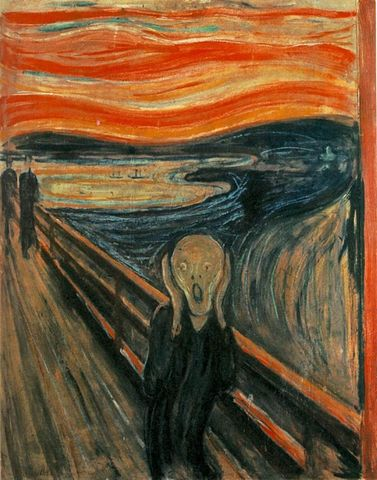
\includegraphics[width=0.9\textwidth]{images/The_Scream.jpg}\end{minipage}
\begin{minipage}[c]{0.55\linewidth}
Marketing of \textit{fear} but :

Double constraint :
\begin{itemize}
\item legally : compatibilities (proprietary licences with free ones, free between them...)
\item technically : security breaches of any external component (HeartBleed in OpenSSL, ...)
\end{itemize}
\end{minipage}

\begin{alertblock}{Security breaches}
Luckily, it was free software....
 \end{alertblock}
 
\end{frame}

\subsection{Tools}

\begin{frame}{Auditing, how ?}

\texttt{grep} and essentially three solutions...

\end{frame}

%%%%%%%%%%%
% BlackDuck
%%%%%%%%%%%%

\begin{frame}{BlackDuck}
  founded by former Microsoft managers.

  \begin{itemize}
  \item Open Source Application Security
  \item Open Source Compliance and Management
  \end{itemize}

\url{https://www.blackducksoftware.com/}
\end{frame}

%%%%%%%%%%%
% FOSSology
%%%%%%%%%%%%

\begin{frame}{FOSSology}

\begin{block}{FOSSology}
\textit{License compliance software system and toolkit.}
\end{block}

\begin{itemize}
\item \textit{As a toolkit you can run license, copyright and export control scans from the command line.}

\item textit{As a system, a database and web ui are provided to give you a compliance workflow. License, copyright and export scanners are tools available to help with your compliance activities.}
\end{itemize}

\url{https://github.com/fossology/fossology}

\end{frame}

\setbeamertemplate{background canvas}{\centering\includegraphics
   [height=\paperheight]{images/fossology-linux-kernel.png}}
\begin{frame}[plain]%{RMS}
%  
\note{FOSSology}
\end{frame}
\setbeamertemplate{background canvas}{}

%%%%%%%%%%%
% Scancode toolkit
%%%%%%%%%%%%

\begin{frame}{Scancode toolkit}
\textit{ ScanCode is a suite of utilities used to scan a codebase for license, copyright, and other interesting information that can be discovered in files.}

\textit{A typical software project often reuses hundreds of third-party components. License and origin information is often scattered and not easy to find: ScanCode discovers this data for you.}

\url{https://github.com/nexB/scancode-toolkit}
\end{frame}

\setbeamertemplate{background canvas}{\centering\includegraphics
   [width=\paperwidth]{images/scancode-ffmpeg.png}}
\begin{frame}[plain]%{RMS}
%  
\note{RMS}
\end{frame}
\setbeamertemplate{background canvas}{}


%%%%%%%%%%%%%%%%%%%%%%%%%%%%%%%%%%%%%%%%%%%%%%%%%%%%%%%%
% Future
%%%%%%%%%%%%%%%%%%%%%%%%%%%%%%%%%%%%%%%%%%%%%%%%%%%%%%%%

\section{Future ?}

\begin{frame}{reciprocity license}

Preliminary : we need qualified legal experts.

  \begin{block}{Problems}
    \begin{itemize}
    \item 70\% of Linux contributions come from just a few big coroporations (name them). 
    \item Wikipedia dépends on Google.
    \item etc
    \item is it still "owned" by the community ? 
    \end{itemize}
  \end{block}

  \begin{block}{What could we do ?}
    \begin{itemize}
    \item "Peer Production license" \textit{(copyfarleft})
    \item "Commons reciprocity license"
    \item "Fair source"
    \item license = wrong path ? Proper laws instead ?
    \end{itemize}
  
  \end{block}
  
 
\end{frame}

\section{Bibliography and credits}

\begin{frame}{References}

Bibliography (in french) :

  \begin{itemize}
  \item "Droit des logiciels, logiciels proprietaires, logiciels libres", F.Pellegrini et S.Canevet, PUF 2013.
  \item "Option libre. Du bon usage des licenses libres", B.Jean, Framabook 2012.
  \item "Histoire et cultures du Libre. Des logiciels partagés aux licenses partagés", Collectif, Framabook 2013.
  \end{itemize}

Websites :

\begin{itemize}
\item \url{http://gplv3.fsf.org/}
\item \url{https://copyleft.org/guide/}
\item \url{http://april.org/en}
\end{itemize}
  
\end{frame}

\begin{frame}{Credits 1/2}
  \begin{itemize}
  \item Photo of Richard Stallman by Lionel Allorge, license GFDL1.3+, CC-BY-SA+, LAL+,  \url{http://photos.april.org/picture.php?/4413/category/159}
  \item Photo of Linus Torvalds from Wikimedia Commons, license CC-BY-SA 3.0 capture d'une vidéo de Linux Foundation Kernel Summit 2008 \url{https://upload.wikimedia.org/wikipedia/commons/3/31/Linus_Torvalds_lks08.jpg}
  \item GNU/Linux, David Revoy, CC-BY \url{http://deevad.deviantart.com/art/GNU-Linux-Portrait-645635708}
  
  \end{itemize}
\end{frame}

\begin{frame}{Credits 2/2}
  \begin{itemize}
\item SMOG grade : Zavras, Alexios (2016) ‘Twenty-five years of school? Analysis of Free and Open Source software license texts’, International Free and Open Source Software Law Review, 8(1), pp 29 – 44 DOI: 10.5033/ifosslr.v8i1.111  
\item Logo GPLv3, license GFDL : \url{http://www.gnu.org/graphics/license-logos.html}
\item The Scream by Edward Munch, Public domain : \url{https://commons.wikimedia.org/wiki/File:The_Scream.jpg}

  \end{itemize}
\end{frame}



\begin{frame}{license}
  Document under GFDL1.3+, CC-BY-SA+, LAL+.
\end{frame}

\end{document}
